







\section{Self paced reading}

In the literature of SA, not much exploratory studies are conducted. Although theoretical explorations are made for what it is \citep{kornfilt1996some,kornfilt2012revisiting,kabak2007turkish,broadwell2008turkish}, not much is done for how it operates except than \cite{kharytonava2012word,kharytonava2012taming} which only investigates a particular type of SA in Turkish compounds. My aim in this experiment is to open up an exploratory field for SA in Turkish with emphasis on language processing. For this purposes I alter the conjoiner and amount of SA in the verbal domain. The reason for choosing only verbal domain for this particular experiment is that there are no ambiguities in the verbal domain SA. Dealing with ambiguities in an experimental setting requires a complicated design for determining dependency resolutions. Although it is a venue that also needs to be explored I reserve the investigation of SA in the nominal domain and its processing for another experiment with an actual language modelling which would enable the testing of the hypotheses of the different approaches. That's why, for the sake of sticking with basic exploratory aspects of SA, I have designed an experiment looking at SA in the verbal domain. In the following subsections I lay out the method, results, and analysis of the experiment.

\subsection{Method}
In this subsection I report the participants, materials, and the procedure for the experiment.

\subsubsection{Participants}

The participants were 160 students at Boğaziçi University who were native speakers of Turkish. In exchange for their participation they have received 1 point to their overall course score on a chosen linguistics course.

\subsubsection{Materials}

The experiment is comprised of three variables. The first variable is the amount of SA with the levels of No SA, One SA, and Full SA. The second variable is the conjoiner with levels \textit{ve} `and' and \textit{veya} `or'. The third variable is contrast. In this variable one of the suspendable suffixes in the second conjunct is altered to have a mismatch between the first and second conjuncts in terms of clause aspect and agreement. This contrast is only performed on the No SA sentence. This way I end up with 3x2 conditions combining the amount of SA and conjoiner type, plus two conditions where I have a contrasting second conjunct for No SA condition with conjoiners. I have made 24 items for the experiment, by 8 conditions I end up with 192 experimental items, I also added 48 filler items. A latin square design by condition is applied, forming 8 lists of 24. This resulted in each participant seeing only 24 experimental items and 48 fillers. All the experimental items have a three word pre and three word post conjunction regions, see the template in (\ref{selfpacedtemplate}). An example set of experimental items with all conditions is given in (\ref{selfpacedexamples}, only relevant parts of the sentence is presented). Half of the items and fillers had yes/no comprehension questions with the correct option being "yes" and the other half had "no" as the correct answer.
\begin{exe}
\ex \label{selfpacedtemplate}
4WORDS CONJ1 \textit{ve/ya} CONJ2 4WORDS
\end{exe}


\begin{exe}
\ex \label{selfpacedexamples}
    \begin{xlist}
     \ex \gll ... yap-sa-ymış-ım ve gönder-se-ymiş-im ... \\ ... do-{\Cond}-{\Prf}-{\First}.{\Sg} {\And} send-{\Cond}-{\Prf}-{\First}.{\Sg} ... \\
     \glt ${}$ \hfill No SA, AND
     
     \ex \gll ... yap-sa-ymış-ım veya gönder-se-ymiş-im ... \\ ... do-{\Cond}-{\Prf}-{\First}.{\Sg} {\And} send-{\Cond}-{\Prf}-{\First}.{\Sg} ... \\
     \glt ${}$ \hfill No SA, OR
     
     \ex \gll ... yap-sa-ymış ve gönder-se-ymiş-im ... \\ ... do-{\Cond}-{\Prf} {\And} send-{\Cond}-{\Prf}-{\First}.{\Sg} ... \\
     \glt ${}$ \hfill One SA, AND
     
     \ex \gll ... yap-sa-ymış veya gönder-se-ymiş-im ... \\ ... do-{\Cond}-{\Prf} {\And} send-{\Cond}-{\Prf}-{\First}.{\Sg} ... \\
     \glt ${}$ \hfill One SA, OR
     
     \ex \gll ... yap-sa ve gönder-se-ymiş-im ... \\ ... do-{\Cond} {\And} send-{\Cond}-{\Prf}-{\First}.{\Sg} ... \\
     \glt ${}$ \hfill Full SA, AND
     
     \ex \gll ... yap-sa veya gönder-se-ymiş-im ... \\ ... do-{\Cond} {\And} send-{\Cond}-{\Prf}-{\First}.{\Sg} ... \\
     \glt ${}$ \hfill Full SA, OR
     
     \ex \gll ... yap-sa-ymış-ız ve gönder-se-ymiş-im ... \\ ... do-{\Cond}-{\Prf}-{\First}.{\Pl} {\And} send-{\Cond}-{\Prf}-{\First}.{\Sg} ... \\
     \glt ${}$ \hfill Contrast, AND
     
     \ex \gll ... yap-sa-ymış-ız veya gönder-se-ymiş-im ... \\ ... do-{\Cond}-{\Prf}-{\First}.{\Pl} {\And} send-{\Cond}-{\Prf}-{\First}.{\Sg} ... \\
     \glt ${}$ \hfill Contrast, OR
    \end{xlist}
\end{exe}

The experiment is formed using http://spellout.net/ibexfarm/ \citep{drummond2013ibex}, and carried out online. For the full list of items and fillers (1-24 and 100-148), see Appendix \ref{selfpaceditems}.

\subsubsection{Procedure}
Participants are provided a link to the experiment prompting them with a consent page. Upon giving consent participants are run through 5 practice items and then they are prompted again for the beginning of the experiment. Each item is presented word by word, and after the end of every sentence a yes/no comprehension question was asked. Participants professed their choice by pushing "Q" key for "yes" and "P" key for "no". After the experiment is done participants are redirected to a separate page to fill their student information to be relayed to the course's professor for extra credit. This is kept separate of the experiment results, protecting participant anonymity.

\subsubsection{Results}
The resulting csv file of the experiment is brought into R \citep{team2013r} for data cleaning, aggregation, and analysis.
The data consisted of 42240 points before cleaning. Two items with a typo, 4 subjects whose accuracies are below 70\% are excluded from the data. After these exclusions, 15.48\% of the trials with incorrect answers are also excluded. The whole cleaning resulted in the loss of 33.33\% of the data.

\begin{figure}[hbt!]
\centering
\begin{knitrout}
\definecolor{shadecolor}{rgb}{0.969, 0.969, 0.969}\color{fgcolor}
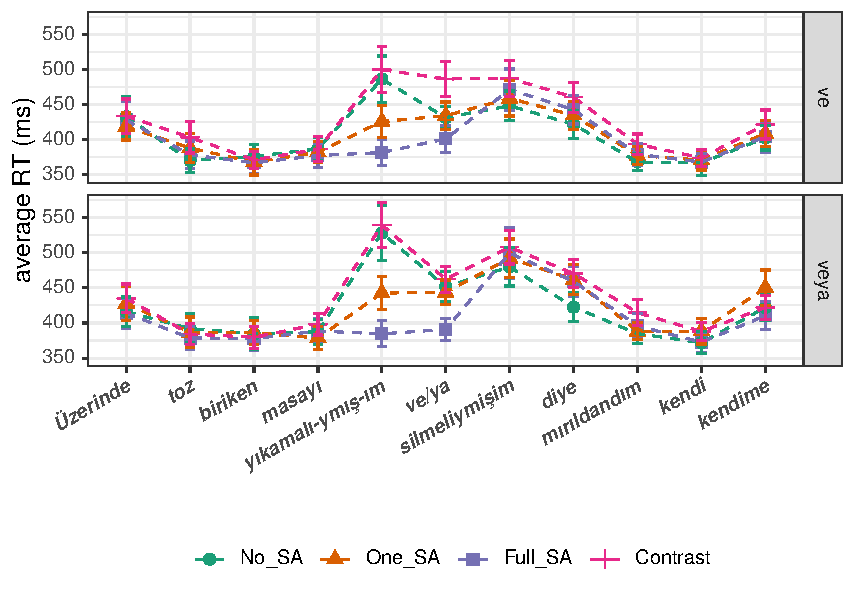
\includegraphics[width=\linewidth]{experiments/selfpaced/report/figure/secondplot-1.pdf} 

\end{knitrout}
\caption{Average reading times for a sentence}
\label{fig:averageRT}
\end{figure}


\begin{figure}[hbt!]
\centering
\begin{knitrout}
\definecolor{shadecolor}{rgb}{0.969, 0.969, 0.969}\color{fgcolor}
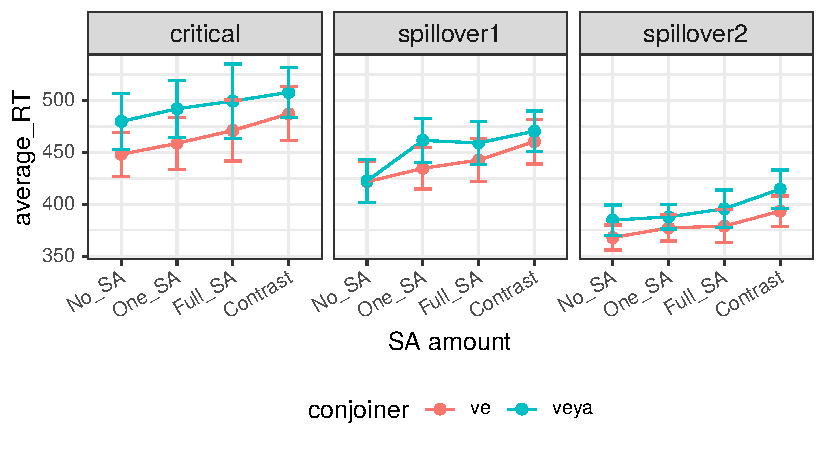
\includegraphics[]{experiments/selfpaced/report/figure/thirdplot-1.pdf} 

\end{knitrout}
\caption{Model results}
\label{fig:modelresults}
\end{figure}

